\documentclass[12pt, twoside]{article}
\usepackage[letterpaper, margin=1in, headsep=0.5in]{geometry}
\usepackage[english]{babel}
\usepackage[utf8]{inputenc}
\usepackage{amsmath}
\usepackage{amsfonts}
\usepackage{amssymb}
\usepackage{tikz}
\usetikzlibrary{quotes, angles}

\usepackage{pgfplots}
\pgfplotsset{width=9cm,compat=1.9}
\usepgfplotslibrary{statistics}
\usepackage{pgfplotstable}

\usepackage{venndiagram}

\usepackage{graphicx}
\usepackage{enumitem}
\usepackage{multicol}
\usepackage{hyperref}

\newif\ifmeta
\metatrue %print standards and topics tags

\title{IB Mathematics}
\author{Chris Huson}
\date{November 2021}

\usepackage{fancyhdr}
\pagestyle{fancy}
\fancyhf{}
\renewcommand{\headrulewidth}{0pt} % disable the underline of the header
\raggedbottom


\fancyhead[LE]{\thepage}
\fancyhead[RO]{\thepage \\ Name: \hspace{4cm} \,\\}
\fancyhead[LO]{BECA / IB Math 02-Descriptive Statistics\\* 19 November 2021}

\begin{document}

\subsubsection*{2.1: Box and whisker plots}
\begin{enumerate}
\item Find the 5-figure summary statistics of the following data (without a calculator):
  \begin{center}
  5 14 3 6 15 11 9 7 14
  \end{center}
  \begin{enumerate}[itemsep=0.7cm]
    \item Rewrite the data in order.
    \item Minimum =
    \item 1st Quartile =
    \item Median =
    \item 3rd Quartile =
    \item Maximum =
    \item Range =
    \item IQR =
  \end{enumerate} \vspace{0.5cm}

\item The box-and-whisker plot represents the examination scores of a group of students.
  \begin{center}
  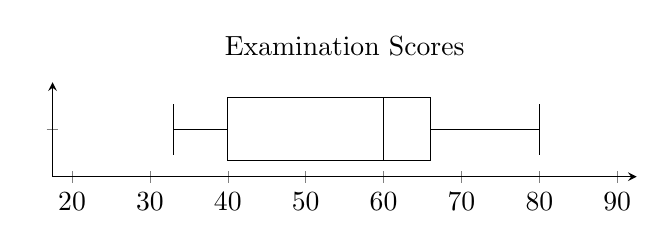
\begin{tikzpicture}[scale=1.0]
    \begin{axis}[
        title={Examination Scores},
        axis lines=left,
        xmin=30, xmax=80,
        y=1cm,
        ytick={1},
        yticklabels={},
      enlargelimits=0.25,
        ]
        %\addplot+ [boxplot]
        %table {3-11_IB-exam.txt};
       \addplot [boxplot prepared={draw position=1,
            lower whisker=33, lower quartile=40,
            median=60,
            upper quartile=66, upper whisker=80,
            %average=28,
            },
        ] coordinates {};
    \end{axis}
    \end{tikzpicture}
  \end{center}
  \begin{enumerate}
    \item Write down each value: \hfill [1 mark]
    \begin{enumerate}
      \begin{multicols}{3}
        \item median =
        \item $Q_1 = $
        \item max =
      \end{multicols}
    \end{enumerate} \vspace{0.5cm}
    The range of the scores is 47 marks, and the interquartile range is 26 marks. \vspace{0.5cm}
    \item Find the value of
    \begin{enumerate}
      \item the minimum score; \hfill [2 marks] \vspace{1cm}
      \item the third quartile. \hfill [2 marks]
    \end{enumerate}
  \end{enumerate}

\newpage
\item Draw a box and whiskers plot of the five-figure summary on the grid. Use a ruler for full credit. \hfill [2 marks] \vspace{0.25cm}\\
min = 2, $Q_1=5$, median = 9, $Q_3=13$, maximum = 16

\begin{center}
  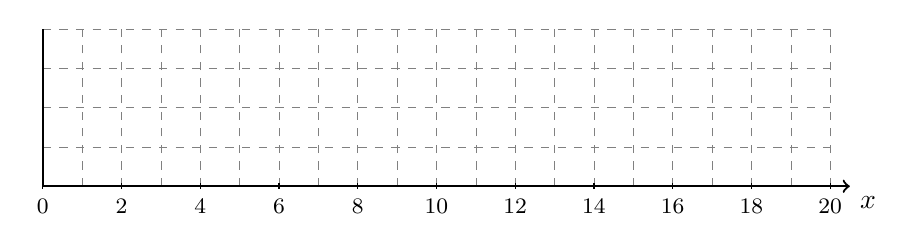
\begin{tikzpicture}[scale=.5]
    \draw [help lines, dashed] (0,0) grid (20,4);
    \draw [thick, ->] (0,0) -- (20.5,0) node [below right] {$x$};
    \foreach \x in {0,2,4,6,8,10, 12, 14, 16, 18, 20}
      \draw[shift={(\x,0)},color=black] (0pt,2pt) -- (0pt,-2pt) node[below] {\footnotesize $\x$};
    \draw [thick, -] (0,0)--(0,4);
  \end{tikzpicture}
\end{center} 

\item Given the following set of 15 data:
    \begin{center}
    3, 4, 4, 5, 5, 5, 6, 8, 9, 11, 11, 15, 15, 16, 17
  \end{center}
  \begin{enumerate}
    \item Write down the mode \hfill [1 marks] \vspace{1cm}
    \item Find the median. \hfill [1 marks] \vspace{1.5cm}
    \item Find the interquartile range. \hfill [2 marks] \vspace{1cm}
    \item Draw a box and whiskers plot of the data on the axis below. \hfill [2 marks] \vspace{1cm}
      \begin{center}
        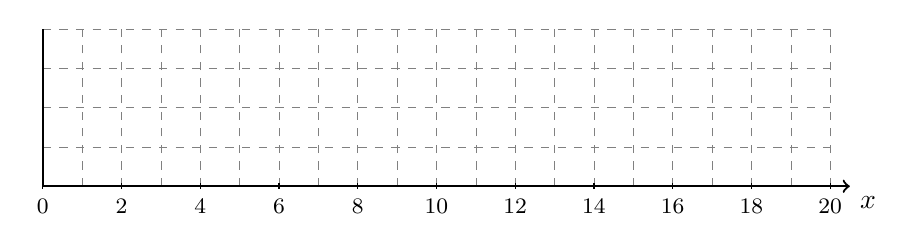
\begin{tikzpicture}[scale=.5]
          \draw [help lines, dashed] (0,0) grid (20,4);
          \draw [thick, ->] (0,0) -- (20.5,0) node [below right] {$x$};
          \foreach \x in {0,2,4,6,8,10, 12, 14, 16, 18, 20}
            \draw[shift={(\x,0)},color=black] (0pt,2pt) -- (0pt,-2pt) node[below] {\footnotesize $\x$};
          \draw [thick, -] (0,0)--(0,4);
        \end{tikzpicture}
      \end{center} \vspace{1cm}
      \item Find the mean. \hfill [2 marks]
    \end{enumerate}

\newpage
\item Consider the following frequency table.
\begin{center}
  \begin{tabular}{|c|c|}
    \hline
    $x$ & Frequency\\ 
    \hline 
    10 & 2 \\ 
    \hline 
    11 & 6 \\ 
    \hline 
    12 & 11 \\ 
    \hline 
    13 & 12 \\ 
    \hline 
    14 & 8 \\ 
    \hline 
    15 & 3 \\ 
    \hline 
    \end{tabular}
\end{center}

\begin{enumerate}
  \item Write down the mode \hfill [1 marks] \vspace{1cm}
  \item Find the value of the range. \hfill [2 marks] \vspace{1.5cm}
  \item Find the value of the mean. \hfill [2 marks] \vspace{1cm}
  \item Find the value of the standard deviation. \hfill [2 marks]
\end{enumerate}
\vspace{1cm}

\item A box contains 100 cards. Each card has a number between one and six written on it. The following table shows the frequencies for each number.
\begin{center}
  \begin{tabular}{|l|r|r|r|r|r|r|}
    \hline
    Number & 1 & 2 & 3 & 4 & 5 & 6\\ 
    \hline 
    Frequency & 26 & 10 & 20 & $k$ & 29 & 11\\ 
    \hline 
  \end{tabular}
\end{center}
\begin{enumerate}
  \item Calculate the value of $k$. \hfill [3 marks] \vspace{1.5cm}
  \item Find
  \begin{enumerate}
    \item the median; \hfill [2 marks] \vspace{2cm}
    \item the interquartile range. \hfill [3 marks]
  \end{enumerate}
\end{enumerate}

\newpage
  \item There are 250 high school students at BECA ranging in age from 13 to 18 years old. The following table shows the frequencies of each age.
    \begin{center}
    \begin{tabular}{|l|r|r|r|r|r|r|}
      \hline
      Age (years) & 13 & 14 & 15 & 16 & 17 & 18\\ 
      \hline 
      Frequency & 27 & 53 & 60 & 55 & 43 & 12\\ 
      \hline 
      \end{tabular}
    \end{center}

  \begin{enumerate}
    %\item Calculate the value of $k$. \hfill [1 mark] \vspace{1.5cm}
    \item Write down the mode. \hfill [1 mark] \vspace{1.5cm}
    \item Find the value of the range. \hfill [1 marks] \vspace{1.5cm}
    \item Find the median. \hfill [1 marks] \vspace{1.5cm}
    \item Find the mean. \hfill [2 marks] \vspace{1.5cm}
    \item Find the standard deviation. \hfill [2 marks] \vspace{1.5cm}
    \item Four years later the same 250 people have moved on to college and career. Find the new values of the 
    \begin{enumerate}
      \item mean; \hfill [1 marks] \vspace{1.5cm}
      \item standard deviation. \hfill [1 marks]
    \end{enumerate}
  \end{enumerate}

\end{enumerate}
\end{document}